\chapter{Dinamika Sitoskeleton dan Gerak Sel}\label{ch:b3:cytoskeleton-motility}

Sebutir neutrofil yang mengejar bakteri melewati jaringan merayap sepuluh
mikrometer tiap menit, dan berganti arah dalam hitungan detik ketika baunya
bergeser. Sebuah vesikel neurotransmiter yang dibuat di dalam badan sel sebuah
neuron motor menempuh satu meter menuruni aksonnya sampai ke kaki, ditarik
sebuah protein motor yang melangkah delapan nanometer, seratus langkah tiap
detik, selama dua minggu. Silia yang melapisi batang tenggorok berdenyut dua
belas kali tiap detik dalam gelombang terselaras yang mengusung debu sehari
naik ke kerongkongan. Semua itu dikerjakan tiga macam filamen protein yang
merakit dan membongkar diri dalam hitungan detik, serta oleh motor yang
membakar satu molekul ATP tiap langkah. Sitoskeleton sama sekali bukan
kerangka dalam arti rangka yang tetap; ia seperangkat polimer yang terus
berganti, dan dinamikanyalah yang \emph{menjadi} mekanisme bentuk, pembelahan,
dan gerak. Bab ini membahas polimernya dan kinetikanya, motornya dan fisika
yang membatasinya, perayapan sebuah sel, serta denyut silia dan flagelum.

\section{Tiga polimer}

\begin{definition}[Filamen aktin, mikrotubulus, filamen antara]\label{def:b3:cytoskeleton-motility:filaments}
\index{filamen aktin}\index{mikrotubulus}\index{filamen antara}%
\index{kepolaran!filamen}\index{sentrosom}
Sebuah \emph{filamen aktin} adalah polimer heliks beruntai dua dari aktin
globular, setebal \qty{7}{nm}, dengan tiap subunitnya \qty{2.7}{nm} sepanjang
sumbunya, dan bersifat polar: ujung \emph{berduri} (plus) tumbuh lebih cepat
daripada ujung \emph{runcing} (minus), dan tiap subunitnya mengusung sebuah ATP
yang dihidrolisis sesudah penyisipannya. Sebuah \emph{mikrotubulus} adalah
tabung berongga bergaris tengah luar \qty{25}{nm} yang dibangun dari tiga belas
protofilamen dimer $\alpha\beta$-tubulin (\qty{8}{nm} tiap dimer), juga polar,
dengan ujung \emph{plus}-nya tumbuh lebih cepat dan ujung \emph{minus}-nya
biasanya tertambat pada \emph{sentrosom} di dekat nukleusnya; subunit
$\beta$-nya menghidrolisis GTP-nya sesudah penyisipan. Sebuah \emph{filamen
antara} adalah tambang setebal \qty{10}{nm} yang terbuat dari protein kumparan
lingkar (keratin di dalam epitelium, vimentin di dalam mesenkim, neurofilamen
di dalam akson, lamin di bawah selubung inti), apolar, tanpa nukleotida, dan
jauh lebih mantap --- yakni kabel penahan tarikan, bukan lintasan yang dinamis.
Aktin sebagian besar duduk di bawah membran plasma dan di dalam tonjolan;
mikrotubulus memancar dari sentrosomnya lalu melayani sebagai lintasan
angkutan jarak jauh dan sebagai gelendongnya; filamen antara memberi sebuah sel
dan nukleusnya ketangguhan mekanisnya.
\end{definition}

\begin{omfigure}
\begin{tikzpicture}[every node/.style={font=\scriptsize}, >=stealth]
  % actin
  \begin{scope}
    \foreach \i in {0,...,11} { \fill[omThm!70] ({\i*0.4},{0.12*sin(\i*60)}) circle (0.17); }
    \node[below, align=center] at (2.2,-0.5) {filamen aktin, \qty{7}{nm}\\heliks beruntai dua, aktin-ATP\\subunit \qty{2.7}{nm} sepanjang sumbunya};
    \node[left] at (-0.3,0) {$-$ runcing}; \node[right] at (4.6,0) {berduri $+$};
  \end{scope}
  % microtubule
  \begin{scope}[xshift=7.2cm]
    \draw[thick, fill=omDef!25] (0,-0.55) rectangle (4.4,0.55);
    \foreach \y in {-0.35,-0.15,0.05,0.25} \draw[omDef] (0,\y) -- (4.4,\y);
    \foreach \x in {0.4,0.8,...,4.0} \draw[omDef] (\x,-0.55) -- (\x,0.55);
    \draw[thick] (4.4,0) ellipse (0.18 and 0.55); \draw[thick, fill=white] (4.4,0) ellipse (0.09 and 0.38);
    \node[below, align=center] at (2.2,-0.65) {mikrotubulus, \qty{25}{nm}\\13 protofilamen $\alpha\beta$-tubulin (GTP)\\dimer sepanjang \qty{8}{nm}};
    \node[left] at (-0.2,0) {$-$}; \node[right] at (4.7,0) {$+$};
  \end{scope}
  % intermediate filament
  \begin{scope}[yshift=-2.9cm, xshift=3.6cm]
    \foreach \dd in {-0.12,0,0.12} \draw[omMeth!70!black, thick] plot[domain=0:4.4, samples=60] (\x, {\dd + 0.1*sin(\x*200 + \dd*400)});
    \node[below, align=center] at (2.2,-0.4) {filamen antara, \qty{10}{nm}\\tambang kumparan lingkar (keratin, vimentin, lamin), tanpa kepolaran, tanpa nukleotida};
  \end{scope}
\end{tikzpicture}

{\small Ketiga filamen itu sesuai skala garis tengahnya. Polimer aktin dan
tubulin bersifat polar dan menghidrolisis sebuah nukleotida sesudah
perakitannya, dan itulah yang membuatnya dinamis; \omterm{def:b3:cytoskeleton-motility:filaments}{filamen antara} adalah
tambang apolar yang dibangun untuk ketahanan.}
\end{omfigure}

\begin{omfigure}
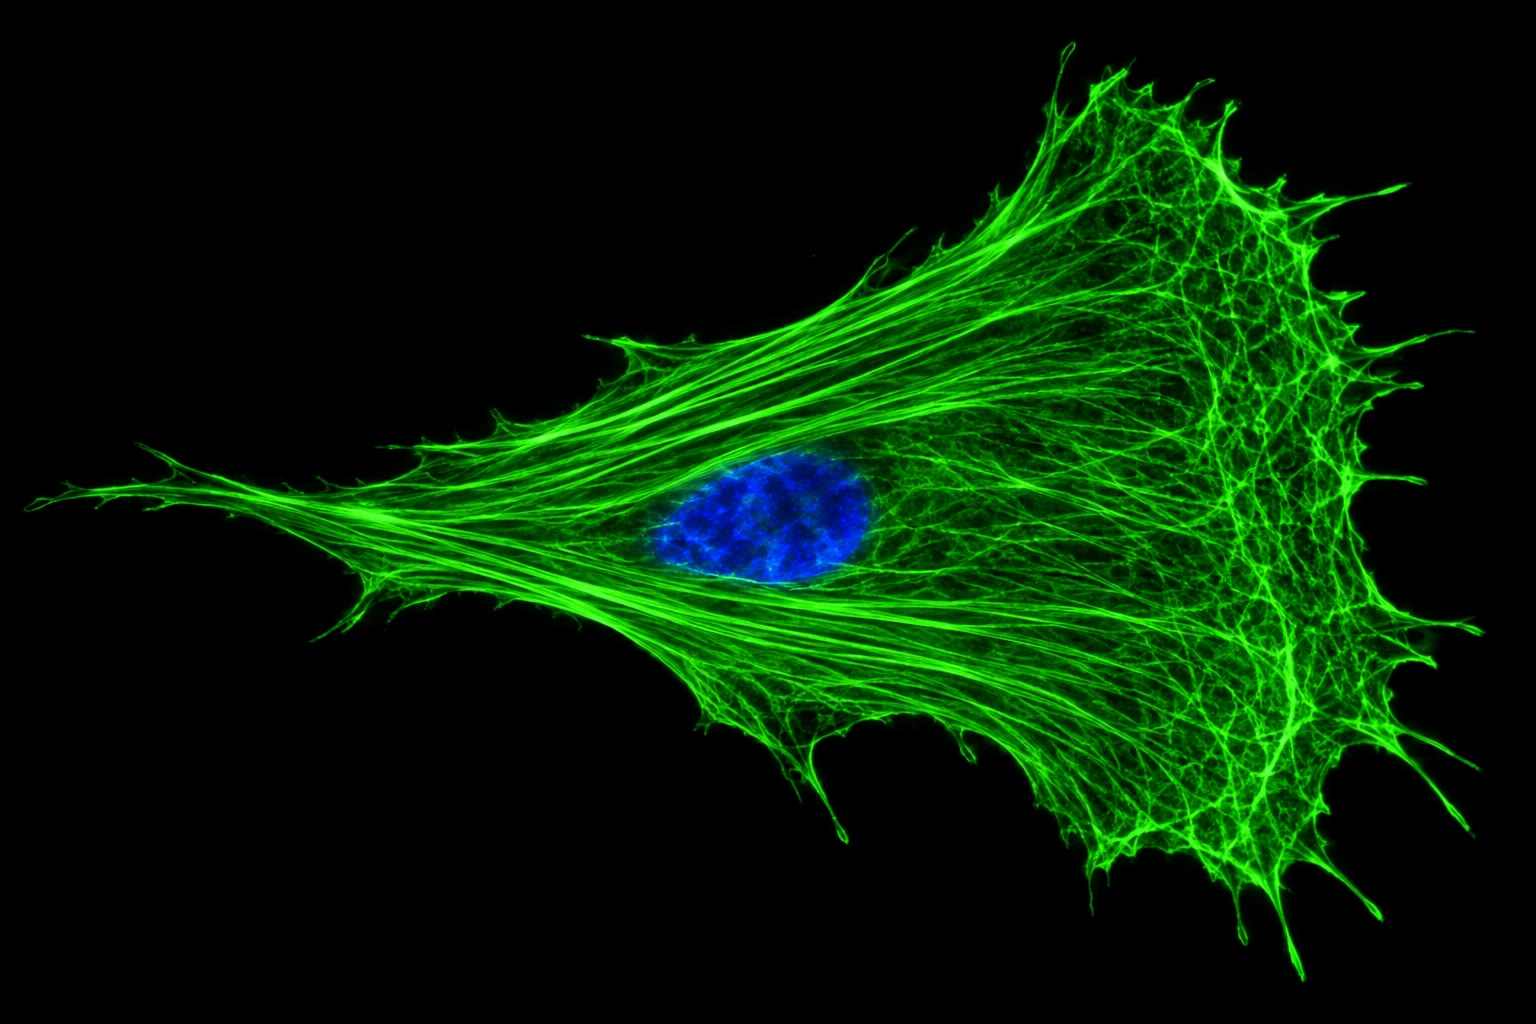
\includegraphics[width=0.54\linewidth]{images/book5/ai/b5-09-fibroblast-actin.jpg}\hspace{0.03\linewidth}
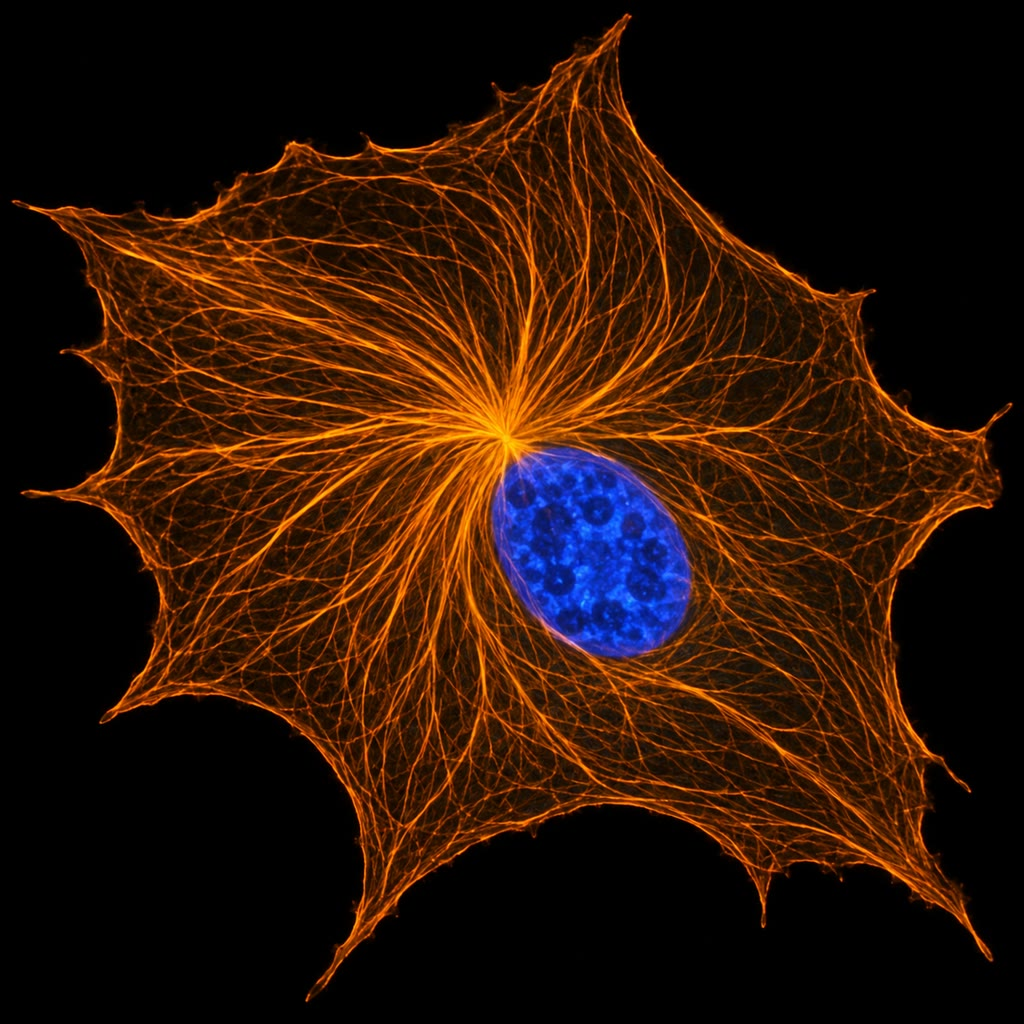
\includegraphics[width=0.36\linewidth]{images/book5/ai/b5-09-microtubules.jpg}

{\small Kiri: aktin (hijau) di dalam fibroblas yang bermigrasi --- serabut
tegangan melintasi tubuhnya, sebuah jala rapat pada tepi depannya yang lebar
di sebelah kanan. Kanan: \omterm{def:b3:cytoskeleton-motility:filaments}{mikrotubulus} (jingga) yang memancar dari \omterm{def:b3:cytoskeleton-motility:filaments}{sentrosom}
di samping nukleusnya (biru) menuju tepi selnya.}
\end{omfigure}

\section{Kinetika sebuah polimer}

\begin{theorem}[Kepekatan kritis dan gerak ban berjalan]\label{thm:b3:cytoskeleton-motility:treadmilling}
\index{kepekatan kritis}\index{gerak ban berjalan}
Misalkan sebuah ujung filamen menambahkan subunit dengan laju $k_{\text{ikat}}C$,
dengan $C$ kepekatan monomer bebasnya, dan kehilangannya dengan laju
$k_{\text{lepas}}$. Ujung itu tumbuh bila $C$ melampaui \emph{\omterm{thm:b3:cytoskeleton-motility:treadmilling}{kepekatan
kritisnya}} $C_{c} = k_{\text{lepas}}/k_{\text{ikat}}$ dan menyusut di bawahnya.
Bila kedua ujungnya berkepekatan kritis berbeda, $C_{c}^{+}
< C_{c}^{-}$, maka pada keadaan tunak ketika filamennya tidak memanjang
maupun memendek kepekatan monomernya adalah
\[
C_{\text{ss}} = \frac{k_{\text{lepas}}^{+} + k_{\text{lepas}}^{-}}
{k_{\text{ikat}}^{+} + k_{\text{ikat}}^{-}},
\qquad C_{c}^{+} < C_{\text{ss}} < C_{c}^{-},
\]
dan ujung plusnya tumbuh sedangkan ujung minusnya menyusut dengan laju yang
sama $J = k_{\text{ikat}}^{+}C_{\text{ss}} - k_{\text{lepas}}^{+} > 0$: subunitnya
mengalir melewati filamennya dari plus ke minus --- itulah \emph{\omterm{thm:b3:cytoskeleton-motility:treadmilling}{gerak ban
berjalan}} --- dengan ongkos satu nukleotida yang terhidrolisis tiap subunit.
\end{theorem}
\begin{proof}
Laju neto pada sebuah ujung adalah $k_{\text{ikat}}C - k_{\text{lepas}}$, dan nol
pada $C_{c}$. Panjang yang tetap menuntut jumlah kedua laju netonya
lenyap, dan hal itu memberi $C_{\text{ss}}$; nilainya terletak di antara kedua
\omterm{thm:b3:cytoskeleton-motility:treadmilling}{kepekatan kritisnya} karena ia rata-rata terbobot keduanya ($C_{\text{ss}} =
(k_{\text{ikat}}^{+}C_{c}^{+} + k_{\text{ikat}}^{-}C_{c}^{-})/(k_{\text{ikat}}^{+}
+ k_{\text{ikat}}^{-})$). Di atas $C_{c}^{+}$ ujung plusnya tumbuh; di bawah
$C_{c}^{-}$ ujung minusnya menyusut; fluksnya adalah laju neto ujung plusnya.
Dua ujung polimer kimia yang sama akan memiliki $C_{c}$ yang sama (tetapan
kesetimbangan yang sama), sehingga adanya selisih menuntut subunitnya berubah
sesudah penyisipan --- yaitu hidrolisis ATP atau GTP --- yang membuat kedua
ujungnya berbeda sekaligus membayar aliran itu.
\end{proof}

\begin{example}[Aktin di dalam tabung reaksi]\label{ex:b3:cytoskeleton-motility:actin-numbers}
Bagi aktin-ATP, $k_{\text{ikat}}^{+} = \qty{11.6}{\micro M^{-1}.s^{-1}}$,
$k_{\text{lepas}}^{+} = \qty{1.4}{s^{-1}}$ ($C_{c}^{+} = \qty{0.12}{\micro
M}$); $k_{\text{ikat}}^{-} = \qty{1.3}{\micro M^{-1}.s^{-1}}$,
$k_{\text{lepas}}^{-} = \qty{0.8}{s^{-1}}$ ($C_{c}^{-} = \qty{0.6}{\micro
M}$). Maka $C_{\text{ss}} = 2.2/12.9 = \qty{0.17}{\micro M}$ dan $J =
11.6\times 0.17 - 1.4 = 0.6$ subunit tiap detik: \qty{1.6}{nm/s},
tak terasakan. Di dalam sel, filamennya bergerak seratus kali lebih cepat,
karena kofilin memutus lalu melucuti aktin-ADP yang lama dari ujung
runcingnya, profilin memuat aktin-ATP yang segar ke ujung berdurinya, dan
protein penudung memutuskan ujung berduri mana yang boleh tumbuh sama sekali:
polimer telanjangnya memasok mekanismenya, pengaturnya memasok kecepatannya.
\end{example}

\begin{omfigure}
\begin{tikzpicture}
\begin{axis}[
  width=0.7\linewidth, height=5.6cm,
  axis x line=bottom, axis y line=left,
  xmin=0, xmax=1.0, ymin=-1.6, ymax=4,
  xlabel={aktin bebas ($\unit{\micro M}$)}, ylabel={laju neto (subunit/s)},
  xlabel style={font=\small, at={(axis description cs:0.5,-0.12)}, anchor=north},
  ylabel style={font=\small},
  tick label style={font=\small}, xtick={0,0.2,0.4,0.6,0.8,1.0}, ytick={-1,0,1,2,3,4},
  clip=false,
]
\addplot[thin, gray, domain=0:1.0, samples=2] {0};
\addplot[very thick, omThm, domain=0:0.46, samples=2] {11.6*x-1.4};
\addplot[very thick, omDef, domain=0:1.0, samples=2] {1.3*x-0.8};
\draw[dashed, gray] (axis cs:0.17,-1.6) -- (axis cs:0.17,4);
\node[font=\scriptsize, omThm, anchor=south east] at (axis cs:0.44,3.1) {ujung berduri};
\node[font=\scriptsize, omDef, anchor=north west] at (axis cs:0.62,-0.25) {ujung runcing};
\node[font=\scriptsize, anchor=south west] at (axis cs:0.19,3.5) {$C_{\text{ss}}$};
\fill[omThm] (axis cs:0.12,0) circle (2pt); \node[font=\scriptsize, anchor=north east] at (axis cs:0.11,-0.05) {$C_{c}^{+}$};
\fill[omDef] (axis cs:0.6,0) circle (2pt); \node[font=\scriptsize, anchor=south west] at (axis cs:0.61,0.05) {$C_{c}^{-}$};
\end{axis}
\end{tikzpicture}

{\small Laju pertumbuhan neto tiap ujung sebuah \omterm{def:b3:cytoskeleton-motility:filaments}{filamen aktin} terhadap
monomer bebasnya, dengan tetapan laju contohnya. Di antara kedua
\omterm{thm:b3:cytoskeleton-motility:treadmilling}{kepekatan kritisnya}, ujung berdurinya tumbuh dan ujung runcingnya
menyusut; pada garis putus-putusnya keduanya tepat saling meniadakan dan
filamennya bergerak seperti ban berjalan.}
\end{omfigure}

\begin{definition}[Ketakmantapan dinamis]\label{def:b3:cytoskeleton-motility:instability}
\index{ketakmantapan dinamis}\index{tudung GTP}\index{bencana}
\omterm{def:b3:cytoskeleton-motility:filaments}{Mikrotubulus} mengerjakan sesuatu yang lebih aneh daripada \omterm{thm:b3:cytoskeleton-motility:treadmilling}{gerak ban berjalan}.
Sebuah ujung plus yang tumbuh mengusung \emph{tudung GTP} berisi dimer yang
baru ditambahkan; di belakangnya GTP-nya dihidrolisis, dan tubulin-GDP, yang
lebih menyukai konformasi melengkung, ditahan tetap lurus di dalam kisinya
dalam keadaan tegang. Bila tudungnya hilang --- ujungnya berhenti sejenak, atau
pertumbuhannya melambat --- protofilamen yang tegang itu mengelupas ke luar
dan \omterm{def:b3:cytoskeleton-motility:filaments}{mikrotubulusnya} memendek pada \qty{300}{nm/s}, yakni dua puluh kali laju
pertumbuhannya: itulah sebuah \emph{bencana}, yang berakhir ketika sebuah dimer
GTP mendarat dan tudung baru terbentuk (sebuah \emph{penyelamatan}). Di dalam
satu populasi, karena itu, sebagian \omterm{def:b3:cytoskeleton-motility:filaments}{mikrotubulus} tumbuh sedangkan tetangganya
runtuh: inilah \emph{ketakmantapan dinamis}. Hal itu memungkinkan sebuah sel
menjelajahi volumenya sendiri dengan ujung plusnya tiap beberapa menit lalu
membangun ulang seluruh lariknya ketika \omterm{def:b3:cytoskeleton-motility:filaments}{sentrosomnya} berpindah atau selnya
membelah. Selnya menalanya lewat protein yang menjejaki ujung plus,
memantapkan (tau, MAP2), memutus (katanin), atau mendepolimerisasi
(kinesin-13) \omterm{def:b3:cytoskeleton-motility:filaments}{mikrotubulusnya}; obat kolkisina dan alkaloid vinka menghalangi
perakitannya sedangkan taksol menghalangi pembongkarannya, dan semuanya racun
gelendong mitosis yang dipakai melawan kanker.
\end{definition}

\begin{proof}[Bukti eksperimental]
Mitchison dan Kirschner (1984) mengamati populasi \omterm{def:b3:cytoskeleton-motility:filaments}{mikrotubulus} yang
ditumbuhkan dari \omterm{def:b3:cytoskeleton-motility:filaments}{sentrosom} di luar sel. Dengan mengencerkan tubulinnya di bawah
\omterm{thm:b3:cytoskeleton-motility:treadmilling}{kepekatan kritisnya}, mereka mengira seluruh \omterm{def:b3:cytoskeleton-motility:filaments}{mikrotubulusnya} akan memendek
perlahan; yang terjadi justru cacah \omterm{def:b3:cytoskeleton-motility:filaments}{mikrotubulusnya} turun sedangkan yang
bertahan terus tumbuh --- sebagian telah membongkar diri sepenuhnya dan cepat,
sebagian lain tidak sama sekali. \omterm{def:b3:cytoskeleton-motility:filaments}{Mikrotubulus} tunggal yang kemudian difilmkan
dengan mikroskopi video beralih mendadak antara fase pertumbuhan yang mantap
dan penyusutan yang cepat. \omterm{def:b3:cytoskeleton-motility:instability}{Tudung GTP} menjelaskan keduanya: hanya ujung yang
bertudung yang tumbuh, dan hilangnya tudung itu peristiwa langka yang bersifat
seluruhnya atau tak sama sekali.
\end{proof}

\section{Motor}

\begin{definition}[Protein motor]\label{def:b3:cytoskeleton-motility:motors}
\index{miosin}\index{kinesin}\index{dinein}\index{keprosesifan}
Sebuah \emph{protein motor} mengubah energi bebas hidrolisis ATP menjadi gerak
yang terarah sepanjang sebuah filamen: \emph{miosin} sepanjang aktin (miosin
II, yakni motor otot dan motor kontraktil, menuju ujung berduri; miosin V,
pengusung vesikel berkepala dua yang melangkah \qty{36}{nm}), \emph{kinesin}
sepanjang \omterm{def:b3:cytoskeleton-motility:filaments}{mikrotubulus} menuju ujung plusnya (kinesin-1 melangkah \qty{8}{nm},
yakni satu dimer tubulin, tiap ATP, tangan berganti tangan, pada kira-kira
\qty{800}{nm/s}), dan \emph{dinein} menuju ujung minusnya (dinein sitoplasma,
bersama adaptornya dinaktin, menghela muatan kembali ke pusat selnya; \omterm{def:b3:cytoskeleton-motility:cilia}{dinein
aksonem} membengkokkan silia). Sebuah motor disebut \emph{prosesif} bila ia
melangkah berkali-kali sebelum terlepas: kinesin-1 berjalan sekitar satu
mikrometer, yakni seratus langkah, sendirian; satu kepala miosin II melakukan
satu sapuan lalu melepaskan diri, sehingga otot menuntut ratusan kepala yang
bekerja pada satu filamen. Motor membaca kepolaran lintasannya, sehingga
geografi sebuah sel --- ujung plus di tepinya, ujung minus di pusatnya ---
menjadi peta tentang ke mana tiap motor akan membawa muatannya.
\end{definition}

\begin{proof}[Bukti eksperimental]
Vale, Reese, dan Sheetz (1985) menemukan \omterm{def:b3:cytoskeleton-motility:motors}{kinesin} sebagai protein aksoplasma
cumi-cumi yang membuat manik lateks meluncur sepanjang \omterm{def:b3:cytoskeleton-motility:filaments}{mikrotubulus} ke arah
plusnya, dan pada tahun-tahun berikutnya struktur berkepala dua, arah tiap
familinya, serta mitra retrogradnya yaitu \omterm{def:b3:cytoskeleton-motility:motors}{dinein} terpilah
satu per satu. Svoboda, Schmidt, Schnapp, dan Block (1993) menahan sebuah manik
yang membawa satu \omterm{def:b3:cytoskeleton-motility:motors}{kinesin} di dalam perangkap optis lalu merekam kedudukannya
dengan daya pisah nanometer: maniknya melaju dalam langkah terpisah sebesar
\qty{8}{nm}, satu langkah tiap ATP pada kepekatan ATP rendah, dan terhenti
melawan gaya sebesar kira-kira \qty{6}{pN}. Tangga molekulnya terlihat
langsung.
\end{proof}

\begin{omfigure}
\begin{tikzpicture}[every node/.style={font=\scriptsize}, >=stealth]
  % left: kinesin on a microtubule
  \begin{scope}
    \draw[thick, fill=omDef!25] (0,0) rectangle (5.4,0.5);
    \foreach \x in {0.4,0.8,...,5.2} \draw[omDef] (\x,0) -- (\x,0.5);
    \node[left] at (-0.1,0.25) {$-$}; \node[right] at (5.5,0.25) {$+$};
    % two heads, stalk, cargo
    \fill[omProp] (2.4,0.72) circle (0.2); \fill[omProp!60] (3.2,0.72) circle (0.2);
    \draw[thick, omProp!80!black] (2.6,0.85) -- (2.85,1.4) -- (3.05,0.85); \draw[thick, omProp!80!black] (2.85,1.4) -- (2.85,2.3);
    \draw[thick, fill=omExo!40] (2.85,2.7) circle (0.4); \node at (2.85,2.7) {muatan};
    \draw[->, thick, omThm] (3.4,0.72) arc[start angle=180, end angle=0, radius=0.4] ; \node[right, omThm] at (3.85,1.15) {\qty{8}{nm} tiap ATP};
    \node[below, align=center] at (2.7,-0.1) {kinesin-1 berjalan tangan berganti tangan menuju ujung plusnya;\\kira-kira $100$ langkah tiap detik, \qty{0.8}{\micro m/s}};
  \end{scope}
  % right: optical trap staircase
  \begin{scope}[xshift=7.2cm, yshift=-0.6cm]
  \begin{axis}[
    width=5.6cm, height=4.4cm, axis lines=left,
    xmin=0, xmax=1.0, ymin=0, ymax=40,
    xlabel={waktu (s)}, ylabel={kedudukan (nm)},
    xlabel style={font=\scriptsize, at={(axis description cs:0.5,-0.12)}, anchor=north},
    ylabel style={font=\scriptsize},
    tick label style={font=\scriptsize}, xtick={0,0.5,1.0}, ytick={0,8,16,24,32},
  ]
  \addplot[very thick, omProp!80!black, const plot] coordinates {(0,0) (0.18,8) (0.31,16) (0.55,24) (0.71,32) (1.0,32)};
  \end{axis}
  \node[font=\scriptsize, align=center] at (2.8,3.6) {satu motor di dalam perangkap optis,\\ATP rendah: langkah \qty{8}{nm}};
  \end{scope}
\end{tikzpicture}

{\small \omterm{def:b3:cytoskeleton-motility:motors}{Kinesin} pada lintasannya dan jejak kakinya di dalam perangkap optis.
Kedua kepalanya berganti-ganti, dan tiap langkahnya memajukan motornya sejauh
satu dimer tubulin, yakni \qty{8}{nm}; pada ATP rendah langkahnya dipisahkan
oleh masa menunggu nukleotida berikutnya dan tangganya terlihat langsung.}
\end{omfigure}

\begin{proposition}[Apa yang diizinkan fisika bagi sebuah motor]\label{prop:b3:cytoskeleton-motility:physics}
\index{gaya henti}\index{energi termal}\index{difusi lawan angkutan}
Hidrolisis satu ATP di dalam sel melepaskan kira-kira \qty{50}{kJ/mol},
yakni $8\times 10^{-20}$ J tiap molekul. Sebuah motor yang maju sejauh $d$
tiap ATP melawan gaya $F$ melakukan kerja $Fd$, sehingga \emph{\omterm{prop:b3:cytoskeleton-motility:physics}{gaya hentinya}}
tak dapat melampaui $F_{\max} = \Delta G/d$: bagi langkah \qty{8}{nm} \omterm{def:b3:cytoskeleton-motility:motors}{kinesin},
nilainya \qty{10}{pN}; angka terukurnya \qty{6}{pN} berarti daya gunanya
mendekati \qty{60}{\%}, lebih tinggi daripada mesin mana pun. \omterm{prop:b3:cytoskeleton-motility:physics}{Energi termal}
$k_{B}T =
4.1\times 10^{-21}$ J, atau \qty{4.1}{pN.nm}, hanya seperdua puluh energi
ATP-nya tetapi diantarkan kepada motornya terus-menerus sebagai tendangan
Brown; sebuah motor adalah alat yang meluruskannya, dengan membiarkan kepalanya
berdifusi maju lalu mengikat ketika kepalanya mendarat, sehingga energi
kimianya dibelanjakan untuk membuat langkahnya tak berbalik, bukan untuk
mendorong. Angkutan oleh motor mengalahkan difusi pada jarak berapa pun yang
berarti di dalam sel yang besar: sebuah vesikel berkoefisien difusi $D = \qty{1}{\micro
m^2/s}$ menuntut waktu $L^{2}/2D$ untuk mengembara sejauh $L$ --- setengah
detik bagi satu mikrometer, tetapi \num{16000} tahun bagi satu meter akson ---
sedangkan sebuah motor pada \qty{1}{\micro m/s} menempuh satu meter itu dalam
dua belas hari.
\end{proposition}
\admitted

\section{Bagaimana sebuah sel merayap}

\begin{definition}[Migrasi sel]\label{def:b3:cytoskeleton-motility:migration}
\index{lamelipodium}\index{kompleks Arp2/3}\index{adhesi fokal}%
\index{integrin}\index{GTPase Rho}
Sebuah sel yang merayap mengulangi daur berisi empat langkah.
\emph{Penonjolan}: pada tepi depannya aktin berpolimerisasi melawan membrannya
sebagai sebuah lembar, yaitu \emph{lamelipodium}, yang jala bercabangnya
dibangun \emph{kompleks Arp2/3}, yang menumbuhkan filamen baru dari sisi
filamen yang sudah ada pada \qty{70}{\degree}, sementara protein penudung
membatasi pertumbuhan tiap filamen dan kofilin mendaur ulang jalanya beberapa
mikrometer di belakangnya; \emph{filopodium} seperti jari yang terbuat dari
filamen terberkas menjajaki ke depan. \emph{Adhesi}: tonjolan barunya melekat
pada alasnya lewat \emph{integrin}, yakni reseptor lintas membran yang mengikat
protein matriks di luarnya dan, lewat protein adaptor, mengikat aktin di
dalamnya, yang mengelompok di dalam \emph{adhesi fokal}. \emph{Kontraksi}:
\omterm{def:b3:cytoskeleton-motility:motors}{miosin} II menarik serabut tegangan yang tertambat pada adhesinya, sehingga
badan selnya terseret maju. \emph{Penarikan}: adhesi di bagian belakangnya
melepaskan diri dan ekornya ditarik masuk. Daurnya diselaraskan tiga \omterm{def:b3:membrane-traffic:coats}{GTPase
kecil} famili \emph{Rho}: Rac menggerakkan lamelipodium, Cdc42 menggerakkan
filopodium, dan Rho menggerakkan serabut tegangan serta kontraksi --- ketiganya
menjadi sasaran reseptor yang membaca arah sebuah landaian kimia
(kemotaksis) atau kekakuan dan pola alasnya.
\end{definition}

\begin{omfigure}
\begin{tikzpicture}[every node/.style={font=\scriptsize}, >=stealth]
  % substrate
  \draw[very thick, gray] (0,0) -- (12,0); \node[below right, gray] at (0,-0.05) {alas (matriks)};
  % cell outline
  \draw[thick, omDef, fill=omDef!10] (1.0,0.05) .. controls (1.2,1.4) and (3.0,2.3) .. (5.0,2.2) .. controls (7.0,2.1) and (8.6,1.4) .. (9.8,0.6) .. controls (10.3,0.4) and (10.8,0.2) .. (11.2,0.05) -- cycle;
  % nucleus
  \draw[thick, fill=omDef!40] (4.6,1.1) ellipse (1.0 and 0.6); \node at (4.6,1.1) {nukleus};
  % lamellipodium: branched actin
  \foreach \p/\a in {(9.9,0.3)/20,(10.1,0.5)/-10,(10.3,0.25)/35,(10.6,0.45)/5,(10.4,0.7)/-25,(9.7,0.7)/15} { \draw[omThm, thick] \p -- ++(\a:0.55); \draw[omThm, thick] \p ++(\a:0.3) -- ++(\a+70:0.35); }
  \node[right, align=left, omThm] at (11.3,1.3) {1. penonjolan:\\aktin bercabang Arp2/3\\mendorong membrannya};
  \draw[->, thick, omThm] (11.3,0.3) -- (11.9,0.3);
  % focal adhesions
  \foreach \x in {9.3,7.6,2.4} \fill[omProp] (\x-0.25,0.03) rectangle (\x+0.25,0.18);
  \node[below, omProp, align=center] at (9.3,-0.45) {2. adhesi: integrin,\\adhesi fokal};
  % stress fibres and myosin
  \foreach \y in {0.45,0.75} \draw[omMeth!70!black, thick] (2.5,\y) -- (7.5,\y+0.1);
  \node[above, omMeth!70!black, align=center] at (7.8,2.3) {3. kontraksi: miosin II\\pada serabut tegangan};
  \draw[->, thick, omMeth!70!black] (6.0,1.55) -- (6.8,1.55);
  % retraction at rear
  \draw[->, thick, gray] (0.8,0.9) -- (1.6,0.9); \node[above, align=center] at (1.4,2.35) {4. penarikan:\\adhesi belakang melepas};
\end{tikzpicture}

{\small Daur perayapannya, dengan arah kiri ke kanan sebagai arah
perjalanannya: polimerisasi aktin yang bercabang mendorong bagian depannya
keluar, \omterm{def:b3:cytoskeleton-motility:migration}{integrin} menambatkannya, \omterm{def:b3:cytoskeleton-motility:motors}{miosin} menarik tubuhnya maju, dan bagian
belakangnya melepaskan diri.}
\end{omfigure}

\begin{example}[Ekor komet Listeria]\label{ex:b3:cytoskeleton-motility:listeria}
Bakteri \emph{Listeria monocytogenes}, begitu berada di dalam sebuah sel,
memajang pada permukaannya satu protein, yaitu ActA, yang merekrut \omterm{def:b3:cytoskeleton-motility:migration}{kompleks
Arp2/3} inangnya. Aktin berpolimerisasi pada permukaan bakterinya lalu
tertinggal di belakang sebagai sebuah ekor; bakterinya terdorong melewati
sitoplasma sampai \qty{0.5}{\micro m/s} dan masuk ke sel tetangganya tanpa
sekali pun meninggalkan sitosolnya. Ekornya adalah \omterm{def:b3:cytoskeleton-motility:migration}{lamelipodium} yang dibalik ke
luar, dengan satu protein di tempat selnya memakai selusin, dan ekor itu
memperlihatkan bahwa polimerisasi aktin saja --- tanpa motor apa pun ---
menghasilkan gaya penonjolannya: tiap subunit yang menyisip di antara jalanya
dan membrannya, ketika sebuah riak termal telah membuka sebuah celah,
meratcet bagian depannya maju sejauh \qty{2.7}{nm}.
\end{example}

\begin{method}[Mengamati pergantian polimernya]\label{met:b3:cytoskeleton-motility:frap}
\index{pemulihan pendaran sesudah fotopemutihan}\index{mikroskopi bintik}
Untuk mengukur dinamika sebuah sistem filamen di dalam sel hidup: (1)
ekspresikanlah subunitnya yang difusikan pada protein berpendar pada kadar
rendah, sehingga subunit itu tersisipkan ke dalam polimer endogennya; (2)
entah pucatkanlah sebuah daerah kecil dengan denyut laser yang kuat lalu
filmkan kembalinya pendarannya seiring subunit yang belum pucat bertukar masuk
(\emph{\omterm{met:b3:cytoskeleton-motility:frap}{pemulihan pendaran sesudah fotopemutihan}}, FRAP) --- waktu paruhnya
adalah waktu tinggal subunitnya, dan bagian yang tak pernah pulih adalah kolam
yang tak bergerak; entah (3) ekspresikanlah subunit berlabel sesedikit mungkin
sehingga polimernya tampak sebagai \emph{bintik} yang jarang, lalu jejakilah:
geraknya adalah aliran ban berjalannya, dan munculnya serta lenyapnya adalah
perakitan dan pembongkarannya. Di dalam sebuah \omterm{def:b3:cytoskeleton-motility:migration}{lamelipodium}, bintiknya mengalir
mundur satu mikrometer tiap menit relatif terhadap alasnya sementara tepinya
maju: jalanya dibangun di depan lalu dihabiskan beberapa mikrometer di
belakangnya.
\end{method}

\section{Silia, flagelum, dan sebuah motor putar}

\begin{definition}[Silia dan flagelum]\label{def:b3:cytoskeleton-motility:cilia}
\index{silium}\index{aksonem}\index{dinein aksonem}%
\index{silium primer}\index{angkutan intraflagelum}
Sebuah \emph{silium} atau \emph{flagelum} eukariot adalah perpanjangan
berselimut membran yang dibangun di atas \emph{aksonem}: sembilan \omterm{def:b3:cytoskeleton-motility:filaments}{mikrotubulus}
ganda dalam sebuah cincin yang mengelilingi sepasang pusat, ditahan kaitan
neksin dan jeruji radial, dan ditumbuhkan dari sebuah badan basal, yakni
sentriol yang termodifikasi. \emph{\omterm{def:b3:cytoskeleton-motility:motors}{Dinein} aksonem} yang melekat pada tiap
gandanya berjalan sepanjang ganda tetangganya menuju ujung minusnya di
pangkalnya; karena gandanya saling terikat, keduanya tak dapat meluncur bebas,
dan luncurannya diubah menjadi bengkokan, yang dirambatkan sepanjang aksonemnya
sebagai gelombang dengan mengalihkan \omterm{def:b3:cytoskeleton-motility:motors}{dinein} yang aktif dari satu sisi cincinnya
ke sisi yang lain. Sebuah silium sepanjang \qtyrange{5}{10}{\micro m}
dan berdenyut \numrange{10}{20} kali tiap detik; sebuah flagelum sperma
sepanjang \qty{50}{\micro m} dan berombak. Protein sebuah silium diusung naik
dari badan selnya oleh kinesin-2 lalu turun oleh dinein-2 sepanjang gandanya,
yakni \emph{angkutan intraflagelum}, dan begitu pula sebuah \emph{silium
primer} yang tak bergerak --- yang hadir, satu tiap sel, pada sebagian besar
sel vertebrata --- dibangun; silium itu sebuah antena indra, yang memuat
reseptor bagi cahaya (segmen luar sel batang), bau, aliran, dan isyarat
perkembangan, dan cacatnya menimbulkan \emph{siliopati}: ginjal polikistik,
kemunduran retina, kegemukan, jari berlebih.
\end{definition}

\begin{omfigure}
\begin{tikzpicture}[every node/.style={font=\scriptsize}, >=stealth]
  % axoneme cross-section
  \begin{scope}
    \draw[thick, omDef!60] (0,0) circle (1.75);
    \foreach \i in {0,...,8} { \begin{scope}[rotate=\i*40] \draw[thick, fill=omDef!30] (0,1.3) circle (0.16); \draw[thick, fill=omDef!30] (0.27,1.22) circle (0.13); \draw[omProp, thick] (0.15,1.05) -- (0.05,0.5); \draw[omThm, thick] (0.4,1.28) -- (0.62,1.2); \end{scope} }
    \draw[thick, fill=omDef!30] (-0.15,0) circle (0.16); \draw[thick, fill=omDef!30] (0.15,0) circle (0.16);
    \node[right, align=left] at (2.0,1.2) {9 mikrotubulus ganda}; \draw (1.9,1.2) -- (1.35,1.0);
    \node[right, align=left] at (2.0,0.4) {sepasang pusat}; \draw (1.9,0.4) -- (0.35,0.1);
    \node[right, align=left, omThm] at (2.0,-0.4) {lengan dinein pada tiap\\ganda menjangkau ganda berikutnya}; \draw[omThm] (1.9,-0.3) -- (1.0,-0.85);
    \node[right, align=left, omProp] at (2.0,-1.3) {jeruji radial}; \draw[omProp] (1.9,-1.3) -- (0.4,-0.7);
    \node[below] at (0,-1.9) {aksonem, selebar \qty{0.25}{\micro m}};
  \end{scope}
  % bending from sliding
  \begin{scope}[xshift=7.6cm]
    \draw[very thick, omDef] (0,-1.6) -- (0,1.6); \draw[very thick, omDef] (0.5,-1.6) -- (0.5,1.6);
    \draw[->, thick, omThm] (0.1,0.5) -- (0.4,0.5); \draw[->, thick, omThm] (0.1,-0.2) -- (0.4,-0.2);
    \node[below, align=center] at (0.25,-1.7) {dinein pada satu ganda\\mendorong tetangganya\\ke arah ujungnya};
    \draw[->, thick] (1.5,0) -- (2.5,0);
    \draw[very thick, omDef] (3.6,-1.6) .. controls (3.6,-0.3) and (4.6,0.5) .. (4.4,1.6); \draw[very thick, omDef] (4.1,-1.6) .. controls (4.1,-0.3) and (5.1,0.5) .. (4.9,1.6);
    \node[below, align=center] at (4.3,-1.7) {terikat pada pangkalnya dan oleh neksin,\\gandanya tak dapat meluncur:\\keduanya membengkok};
  \end{scope}
\end{tikzpicture}

{\small \omterm{def:b3:cytoskeleton-motility:cilia}{Aksonem} dalam penampang lintang (kiri): sembilan ganda mengelilingi
sepasang pusat, dengan lengan \omterm{def:b3:cytoskeleton-motility:motors}{dinein} dan jeruji radial. Kanan: \omterm{def:b3:cytoskeleton-motility:motors}{dinein}
meluncurkan satu ganda sepanjang ganda berikutnya, dan karena gandanya
tertambat, luncurannya menjadi bengkokan yang merambat sepanjang \omterm{def:b3:cytoskeleton-motility:cilia}{siliumnya}.}
\end{omfigure}

\begin{omfigure}
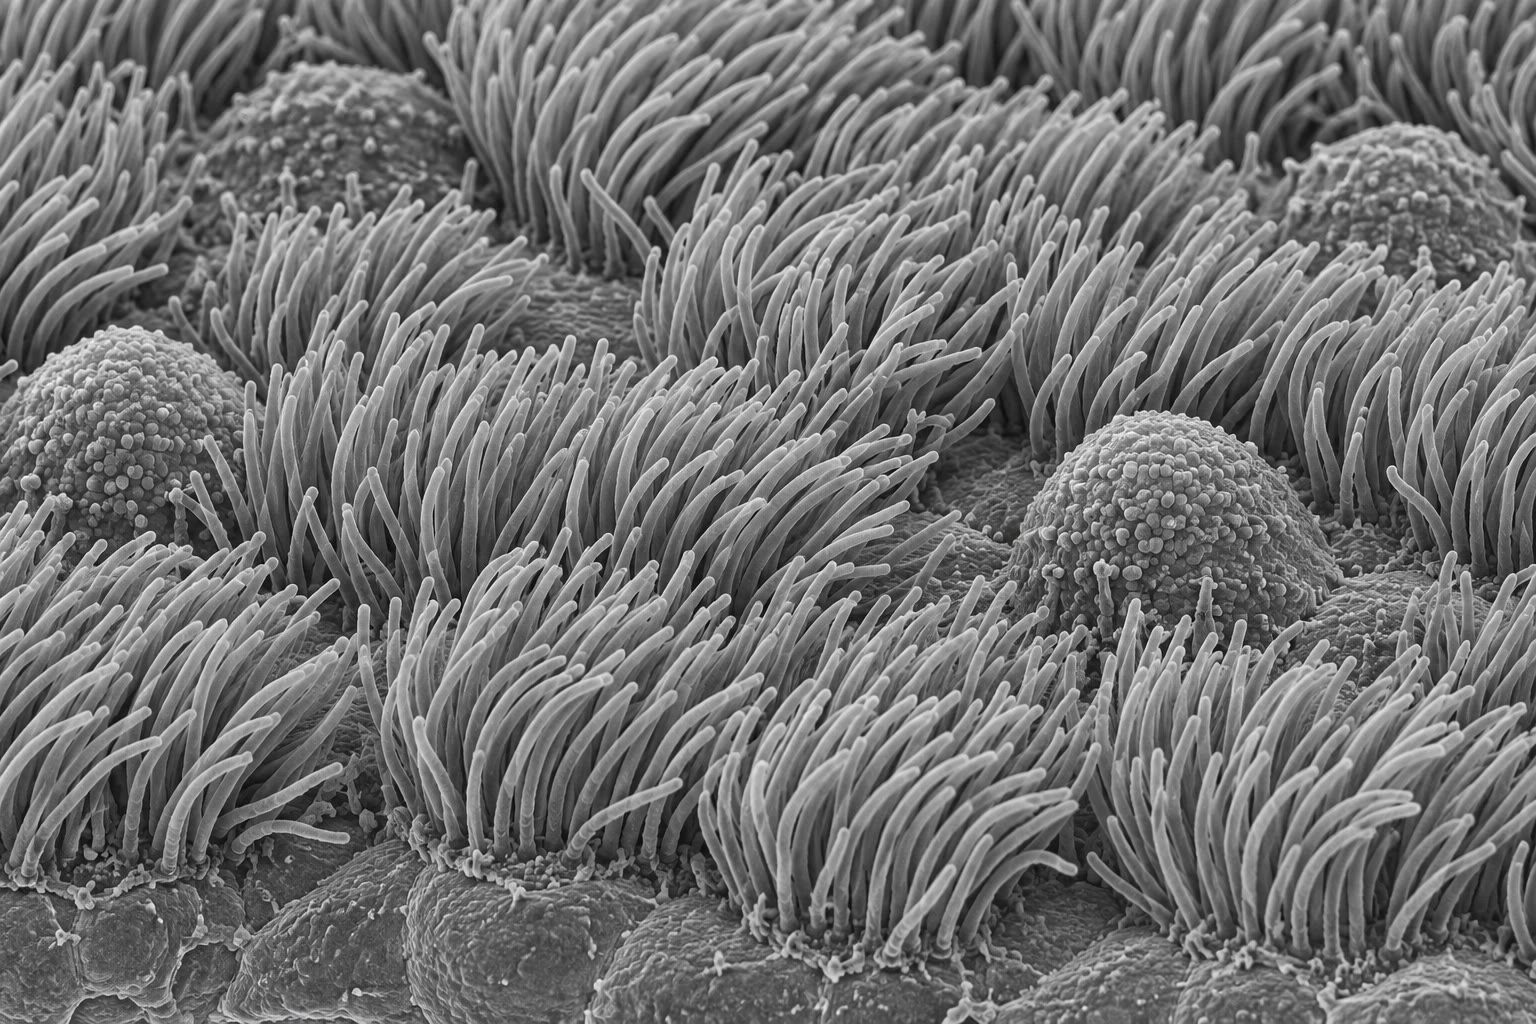
\includegraphics[width=0.54\linewidth]{images/book5/ai/b5-09-cilia-sem.jpg}\hspace{0.03\linewidth}
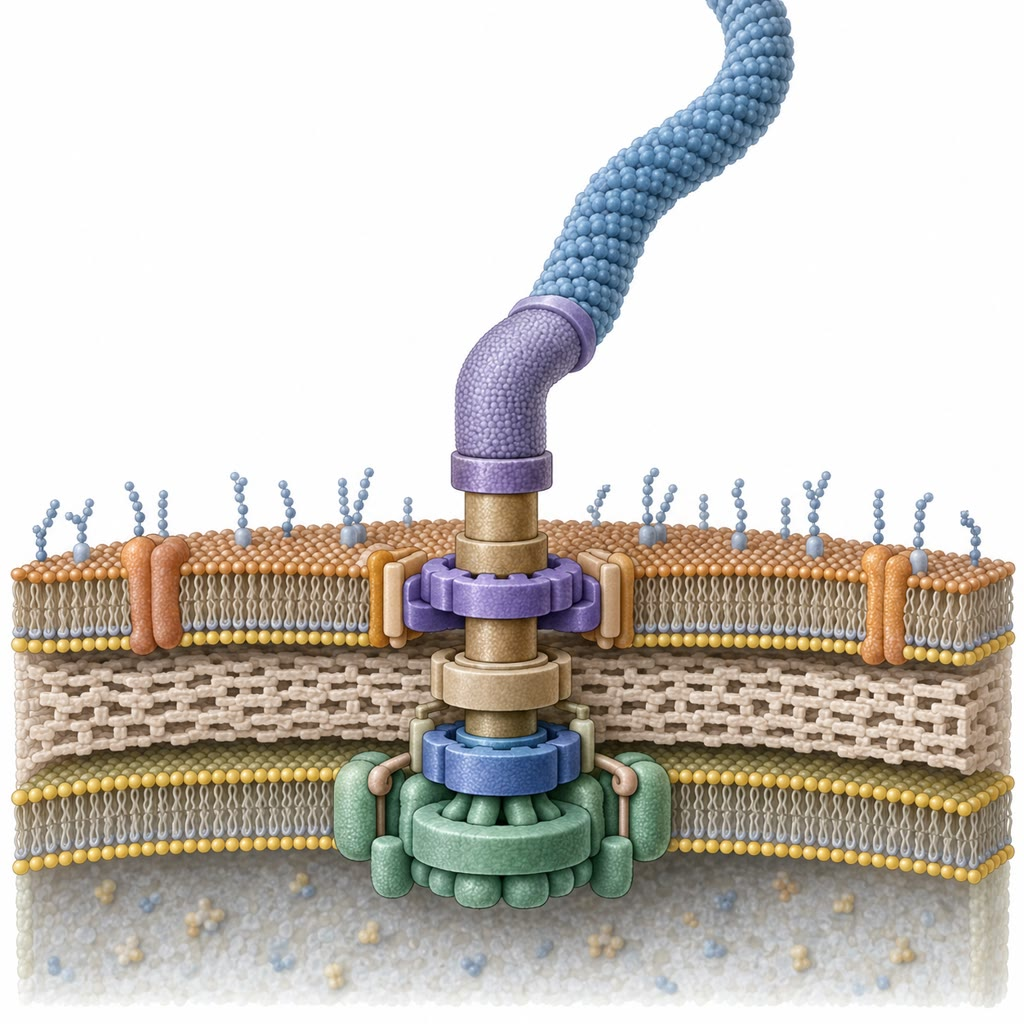
\includegraphics[width=0.36\linewidth]{images/book5/ai/b5-09-flagellar-motor.jpg}

{\small Kiri: epitelium bersilia trakea di bawah mikroskop
elektron payar, yakni hamparan silia di antara sel penyekresi lendir yang
berbentuk kubah. Kanan: \omterm{prop:b3:cytoskeleton-motility:flagellar-motor}{motor flagelum} bakteri, yakni mesin putar berisi cincin
di dalam selubung selnya yang digerakkan aliran proton.}
\end{omfigure}

\begin{proposition}[Motor flagelum bakteri]\label{prop:b3:cytoskeleton-motility:flagellar-motor}
\index{motor flagelum}\index{lari dan jungkir}
Flagelum bakteri tak berkerabat dengan flagelum eukariot: ia filamen heliks
yang kaku dari flagelin, setebal \qty{20}{nm} dan sepanjang beberapa
mikrometer, yang diputar sebuah \emph{motor putar} yang terbenam di dalam
selubung selnya --- sebuah rotor berisi sekitar empat puluh lima protein yang
dikelilingi cincin satuan stator, dan masing-masing satuan itu sebuah saluran
tempat proton mengalir menuruni landaiannya ke dalam selnya, kira-kira seribu
proton tiap putaran. Motornya berputar sampai \qty{300}{Hz}, membalik arah
dalam satu milidetik, dan membangkitkan torsi sekitar \qty{1000}{pN.nm}; ia
dibangun dari kira-kira dua puluh protein yang gennya dinyalakan menurut
urutan perakitan bagiannya, dari dalam ke luar. Pada \emph{E.~coli},
perputaran berlawanan arah jarum jam memberkas beberapa flagelumnya menjadi
sebuah baling-baling dan selnya \emph{berlari} lurus; peralihan ke arah jarum
jam menerbangkan berkasnya berantakan dan selnya \emph{berjungkir} ke arah acak
yang baru. Lintasan kemotaksisnya tidak membiaskan apa pun selain frekuensi
jungkirnya --- lebih jarang ketika keadaannya membaik --- dan hal itu sudah
memadai untuk mendaki sebuah landaian.
\end{proposition}

\begin{remark}[Sitoskeleton adalah sebuah kata kerja]\label{rem:b3:cytoskeleton-motility:verb}
Nyaris tak ada yang diuraikan bab ini merupakan struktur dalam arti sebuah
tulang: \omterm{def:b3:cytoskeleton-motility:migration}{lamelipodiumnya} adalah gelombang polimerisasi, gelendong
\cref{ch:b3:cell-cycle-apoptosis} adalah keadaan tunak \omterm{def:b3:cytoskeleton-motility:filaments}{mikrotubulus} yang
tumbuh dan runtuh, dan denyut \omterm{def:b3:cytoskeleton-motility:cilia}{siliumnya} adalah pola peralihan motor.
Pergantiannya bukan ongkos yang ditoleransi selnya melainkan mekanismenya
sendiri, dan itulah sebabnya setiap sistem ini berjalan atas hidrolisis
nukleotida lalu berhenti dalam hitungan menit sesudah ATP-nya menipis, dan
sebabnya racun yang membekukan polimernya pada keadaan mana pun --- taksol atau
kolkisina, faloidin atau sitokalasin --- sama mematikannya.
\end{remark}

\section{Latihan}

\begin{exercise}[$\star$]\label{exo:b3:cytoskeleton-motility:1}
Bandingkanlah \omterm{def:b3:cytoskeleton-motility:filaments}{filamen aktin}, \omterm{def:b3:cytoskeleton-motility:filaments}{mikrotubulus}, dan \omterm{def:b3:cytoskeleton-motility:filaments}{filamen antara} menurut
garis tengah, subunit, kepolaran, nukleotida, dan peran lazimnya.
\end{exercise}

\begin{exercise}[$\star$]\label{exo:b3:cytoskeleton-motility:2}
Definisikanlah \omterm{thm:b3:cytoskeleton-motility:treadmilling}{kepekatan kritis}. Mengapa kedua ujung sebuah \omterm{def:b3:cytoskeleton-motility:filaments}{filamen aktin}
berkepekatan kritis berbeda, dan apa yang akan terjadi
bila keduanya sama?
\end{exercise}

\begin{exercise}[$\star$]\label{exo:b3:cytoskeleton-motility:3}
Sebutkanlah satu motor bagi masing-masing: vesikel menuju tepi selnya pada
\omterm{def:b3:cytoskeleton-motility:filaments}{mikrotubulus}; vesikel menuju pusatnya; kontraksi sebuah serabut
tegangan; pembengkokan sebuah \omterm{def:b3:cytoskeleton-motility:cilia}{silium}. Berikanlah arah yang diambil
masing-masing pada lintasannya.
\end{exercise}

\begin{exercise}[$\star$]\label{exo:b3:cytoskeleton-motility:4}
Sebutkanlah keempat langkah daur perayapannya dan GTPase famili Rho
yang mengaturnya pada tiga langkah yang pertama.
\end{exercise}

\begin{exercise}[$\star\star$]\label{exo:b3:cytoskeleton-motility:5}
Sebuah ujung plus polimer memiliki $k_{\text{ikat}} = \qty{5}{\micro M^{-1}.s^{-1}}$,
$k_{\text{lepas}} = \qty{1}{s^{-1}}$, dan ujung minusnya $k_{\text{ikat}} =
\qty{1}{\micro M^{-1}.s^{-1}}$, $k_{\text{lepas}} = \qty{0.8}{s^{-1}}$.
Carilah kedua \omterm{thm:b3:cytoskeleton-motility:treadmilling}{kepekatan kritisnya}, kepekatan tunaknya,
dan laju \omterm{thm:b3:cytoskeleton-motility:treadmilling}{gerak ban berjalannya} dalam subunit tiap detik dan, bagi
subunit \qty{2.7}{nm}, dalam nanometer tiap detik.
\end{exercise}

\begin{exercise}[$\star\star$]\label{exo:b3:cytoskeleton-motility:6}
\omterm{def:b3:cytoskeleton-motility:motors}{Kinesin} berjalan pada \qty{800}{nm/s} dengan langkah \qty{8}{nm}, satu ATP
masing-masing. Berapa ATP tiap detik tiap motornya? Akson sebuah neuron
sepanjang \qty{1}{m}: berapa lama perjalanannya, dan berapa ATP yang
dibelanjakan satu motor untuk itu? Bandingkanlah
dengan waktu difusi \cref{prop:b3:cytoskeleton-motility:physics}.
\end{exercise}

\begin{exercise}[$\star\star$]\label{exo:b3:cytoskeleton-motility:7}
\omterm{def:b3:cytoskeleton-motility:motors}{Miosin} V melangkah \qty{36}{nm} tiap ATP. Berapa \omterm{prop:b3:cytoskeleton-motility:physics}{gaya henti} maksimumnya,
dan mengapa nilainya lebih rendah daripada milik \omterm{def:b3:cytoskeleton-motility:motors}{kinesin}? Motor yang mana yang
lebih cocok mengusung muatan besar, dan yang mana untuk bergerak cepat?
\end{exercise}

\begin{exercise}[$\star\star$]\label{exo:b3:cytoskeleton-motility:8}
Ramalkanlah pengaruhnya pada sel yang membelah, dan pada sel yang merayap, dari
(a) taksol, (b) kolkisina, (c) sitokalasin, (d) sebuah penghambat Rac, lalu
jelaskan masing-masing dari mekanismenya.
\end{exercise}

\begin{exercise}[$\star\star$]\label{exo:b3:cytoskeleton-motility:9}
Pada sebuah percobaan FRAP atas \omterm{def:b3:cytoskeleton-motility:migration}{lamelipodium}, pendarannya pulih dengan
waktu paruh \qty{20}{s} sampai \qty{90}{\%} nilai awalnya. Berapa
waktu tinggal aktin di dalam jalanya dan berapa bagian yang tak bergerak?
Bintiknya mengalir mundur pada \qty{1.5}{\micro m/min} sementara tepinya
maju pada \qty{1}{\micro m/min}: pada laju berapa aktinnya berpolimerisasi
pada tepinya?
\end{exercise}

\begin{exercise}[$\star\star\star$]\label{exo:b3:cytoskeleton-motility:10}
Jelaskanlah \omterm{def:b3:cytoskeleton-motility:instability}{ketakmantapan dinamis} dari segi \omterm{def:b3:cytoskeleton-motility:instability}{tudung GTP}, lalu tunjukkan mengapa
populasi \omterm{def:b3:cytoskeleton-motility:filaments}{mikrotubulus} yang ditahan tepat di atas \omterm{thm:b3:cytoskeleton-motility:treadmilling}{kepekatan kritisnya}
menjadi bimodal panjangnya, bukan seragam. Apa yang diperoleh selnya
dari perilaku yang memboroskan GTP itu?
\end{exercise}

\begin{exercise}[$\star\star\star$]\label{exo:b3:cytoskeleton-motility:11}
Sebuah bakteri sepanjang \qty{2}{\micro m} berenang pada \qty{25}{\micro m/s}.
Di dalam air pada skala ini seretan kental mendominasi dan selnya berhenti
dalam jarak satu nanometer ketika motornya berhenti. Jelaskanlah mengapa gerak
bolak-balik (sebuah dayung) tak dapat mendorongnya sedangkan heliks yang
berputar dapat, lalu taksirlah cacah proton yang dibelanjakan motornya tiap
detik pada \qty{100}{Hz}.
\end{exercise}

\begin{exercise}[$\star\star\star$]\label{exo:b3:cytoskeleton-motility:12}
Sindrom Kartagener --- silia yang tak bergerak --- memberi bronkitis menahun,
kemandulan pria, dan pada separuh pasiennya sebuah jantung di sisi kanan.
Jelaskanlah masing-masing dari biologi \omterm{def:b3:cytoskeleton-motility:cilia}{aksonemnya}, lalu katakan mengapa yang
terakhir hanya mengenai separuhnya.
\end{exercise}

\section{Soal: Sebutir Neutrofil yang Bergerak}

\begin{problem}[{Soal akhir pekan --- anggaran aktin sebutir neutrofil yang
dicacah, gerak ban berjalannya yang dihitung, perjalanan sebuah vesikel
menuruni akson yang ditakar terhadap difusi, daya guna sebuah motor yang
diukur, serta polimerisasi dan ongkos ATP bagian depan perayapannya, berakhir
pada laju gerak ban berjalannya, waktu menyeberangi sebuah akson, dan ATP yang
dibakar sebuah lamelipodium tiap detik}]
\label{pb:b3:cytoskeleton-motility:1}
Data: sebutir neutrofil bervolume \qty{300}{\micro m^3} memuat aktin pada
\qty{200}{\micro M}, separuhnya terpolimerisasi; sebuah subunit menambahkan
\qty{2.7}{nm} pada sebuah filamen. Tetapan laju aktinnya seperti pada
\cref{ex:b3:cytoskeleton-motility:actin-numbers}. \omterm{def:b3:cytoskeleton-motility:motors}{Kinesin}: langkah
\qty{8}{nm}, \qty{800}{nm/s}, \omterm{prop:b3:cytoskeleton-motility:physics}{gaya henti} \qty{6}{pN}; hidrolisis ATP
$\Delta G = \qty{50}{kJ/mol}$; $k_{B}T = \qty{4.1}{pN.nm}$; koefisien difusi
vesikelnya \qty{1}{\micro m^2/s}; panjang aksonnya \qty{1}{m}.
\omterm{def:b3:cytoskeleton-motility:migration}{Lamelipodiumnya} selebar \qty{20}{\micro m} dengan $200$ filamen tiap
mikrometer tepinya, yang maju pada \qty{10}{\micro m/min}; jalanya
dibongkar \qty{3}{\micro m} di belakang tepinya.

\medskip
\noindent\textbf{Bagian I --- Anggaran aktinnya.}
\begin{enumerate}
  \item Berapa molekul aktin yang dikandung selnya, dan berapa yang
        berada di dalam filamen?
  \item Berapa panjang filamen seluruhnya? Bila filamen rata-ratanya
        \qty{0.25}{\micro m}, berapa filamennya?
  \item Aktin bebasnya \qty{100}{\micro M}, jauh di atas \omterm{thm:b3:cytoskeleton-motility:treadmilling}{kepekatan
        kritis} ujung berdurinya. Mengapa filamennya tidak begitu saja
        tumbuh sampai monomernya habis? (Dua protein.)
  \item \omterm{thm:b3:cytoskeleton-motility:treadmilling}{Gerak ban berjalan} di luar sel: hitunglah $C_{\text{ss}}$ dan $J$ dari
        tetapan lajunya, dan laju \omterm{thm:b3:cytoskeleton-motility:treadmilling}{gerak ban berjalannya} dalam nanometer tiap
        detik dan mikrometer tiap menit.
  \item Di dalam selnya laju efektifnya \qty{1}{\micro m/min}. Dengan
        faktor berapa pengaturnya mempercepat polimer telanjangnya?
  \item Tiap subunit yang bergerak seperti ban berjalan memakan satu ATP. Bila
        seluruh $2\times 10^{5}$ filamennya bergerak pada laju selulernya,
        berapa ATP tiap detik, dan berapa bagiannya dari pergantian total
        sebuah sel yang sekitar $10^{9}$ ATP tiap detik?
\end{enumerate}

\medskip
\noindent\textbf{Bagian II --- Sebuah vesikel menuruni akson.}
\begin{enumerate}[resume]
  \item Berapa lama sebuah vesikel yang digerakkan \omterm{def:b3:cytoskeleton-motility:motors}{kinesin} menempuh aksonnya,
        dan berapa langkah serta ATP yang dibelanjakan motornya?
  \item Berapa lama difusi memakan waktu sepanjang \qty{1}{m}? Sepanjang
        \qty{10}{\micro m}, yakni lebar sebuah badan sel? Apa yang dikatakan
        perbandingan itu tentang di mana sel masih sanggup mengandalkan
        difusi?
  \item Hitunglah energi tiap ATP dalam joule dan dalam satuan $k_{B}T$.
  \item Berapa gaya maksimum sebuah motor berlangkah \qty{8}{nm}, dan berapa
        daya guna \omterm{def:b3:cytoskeleton-motility:motors}{kinesin} pada keadaan henti?
  \item Sebuah vesikel berjari-jari \qty{100}{nm} di dalam sitoplasma
        berkekentalan \qty{0.01}{Pa.s} (sepuluh kali air) yang bergerak pada
        \qty{800}{nm/s} merasakan seretan $F = 6\pi\eta r v$. Hitunglah
        seretan itu, lalu bandingkan dengan \omterm{prop:b3:cytoskeleton-motility:physics}{gaya hentinya}: berapa motor yang
        dibutuhkan?
  \item Akson sebuah neuron mengusung sekitar $10^{4}$ vesikel sekaligus.
        Berapa konsumsi ATP total angkutannya tiap detik, dan bagaimana
        perbandingannya dengan ongkos penyalaan neuronnya yang sekitar
        $10^{9}$ ATP tiap detik? Apa yang tersirat dari hal itu bagi sebuah
        neuron yang mitokondrianya gagal?
\end{enumerate}

\medskip
\noindent\textbf{Bagian III --- Bagian depannya.}
\begin{enumerate}[resume]
  \item Ubahlah laju tepinya menjadi nanometer tiap detik, lalu hitunglah
        cacah subunit tiap detik yang harus ditambahkan tiap filamen agar
        mengimbangi.
  \item Berapa filamen yang mendorong tepinya, dan berapa subunit tiap
        detik yang dihabiskan seluruh tepinya?
  \item Tiap subunit yang ditambahkan adalah satu ATP yang dihidrolisis lalu
        kemudian didaur ulang. Berapa ATP tiap detik bagi penonjolannya;
        berapa bagiannya dari $10^{9}$ tiap detik milik selnya?
  \item Jala di belakang tepinya sedalam \qty{3}{\micro m} dan dibongkar
        di situ. Berapa umur sebuah subunit di dalam jalanya, dan berapa
        subunit yang berada di dalam jalanya pada tiap saat?
  \item Membrannya melawan penonjolan dengan gaya sekitar
        \qty{1}{pN} tiap filamen. Hitunglah kerja yang dilakukan tiap subunit
        yang ditambahkan ($F\times \qty{2.7}{nm}$) dalam $k_{B}T$ lalu katakan
        apakah ratcet Brown --- sebuah riak termal yang membuka celah
        \qty{2.7}{nm} --- masuk akal.
  \item Mengapa ekor komet Listeria tak menuntut motor, dan secepat apa
        ekor itu dapat mendorong bila ia merekrut permesinan yang sama?
\end{enumerate}

\medskip
\noindent\textbf{Bagian IV --- Arah.}
\begin{enumerate}[resume]
  \item Neutrofilnya mengindera sebuah penarik kimia yang kepekatannya
        naik \qty{2}{\%} sepanjang lebarnya \qty{10}{\micro m}. Dengan
        \num{50000} reseptor dan $K_{d}$ sama dengan kepekatan
        rata-ratanya, berapa reseptor lagi yang terisi pada separuh bagian
        depannya dibandingkan separuh bagian belakangnya? (Keterisiannya
        $\theta = C/(C +
        K_{d})$; pakailah separuh reseptornya tiap sisi.)
  \item Riak acak cacah yang terisi pada satu sisinya kira-kira akar
        kuadrat cacahnya. Apakah selisih pertanyaan 19 terdeteksi pada satu
        saat tunggal? Bagaimana perata-rataan sepanjang beberapa detik
        membantunya?
  \item GTPase yang mana yang harus diaktifkan di depan dan yang mana di
        belakang agar selnya berbelok ke arah sumbernya? Apa yang akan
        dilakukan sebuah sel yang Rac-nya aktif terus-menerus di mana-mana?
  \item Selnya mencapai bakterinya dalam \qty{3}{min} dari jarak
        \qty{30}{\micro m}. Periksalah lajunya terhadap datanya.
  \item Sebuah sel yang tak memiliki Arp2/3 bergerak dengan menggelembung ---
        yakni tonjolan membran yang digerakkan tekanan --- sebagai gantinya.
        Langkah mana pada daurnya yang telah tergantikan, dan apa yang
        dikatakannya tentang peran aktin pada langkah yang lain?
  \item Seluruh daur perayapannya memakan beberapa menit, namun selnya
        berbelok dalam hitungan detik ketika landaiannya bergeser.
        Jelaskanlah, dengan memakai umur jalanya dari pertanyaan~16.
  \item Ringkaskanlah: laju \omterm{thm:b3:cytoskeleton-motility:treadmilling}{gerak ban berjalan} di luar sel (pertanyaan~4),
        waktu sebuah vesikel menempuh aksonnya (pertanyaan~7), dan ATP
        tiap detik yang dibelanjakan bagi penonjolannya (pertanyaan~15).
\end{enumerate}
\end{problem}
